%!TEX root = htm.tex
\section{Evaluation}
\label{sec:eval}
%
In this section, we study the performance characteristics of Algorithms~\ref{alg:inswrite} and \ref{alg:inswrite2}, Hybrid NOrec, TLE and TL2.
Our experimental goals are (G1) to study the performance impact of instrumentation on the fast-path and validation on the slow path, 
(G2) to understand how Algorithms~\ref{alg:inswrite} and \ref{alg:inswrite2} perform relative to the other algorithms,
(G3) the impact of HyTM algorithm design on the performance in Intel and IBM Power8 HTMs, and 
(G4) to determine whether direct accesses can be used to obtain significant performance improvements on IBM Power8 using the supported suspend/resume isntruction to escape from a hardware transaction.

\vspace{1mm}\noindent\textbf{Experimental system (Intel).}
The experimental system is a large-scale 2-socket Intel E7-4830 v3 with 12 cores per socket and 2 hyperthreads (HTs) per core, for a total of 48 threads.
Each core has a private 32KB L1 cache and 256KB L2 cache (which is shared between HTs on a core).
All cores on a socket share a 30MB L3 cache.
This system has a non-uniform memory architecture (NUMA) in which threads have significantly different access costs to different parts of memory depending on which processor they are currently executing on.

We pin threads so that the first socket is saturated before we place any threads on the second socket.
Thus, thread counts 1-24 run on a single socket.
Furthermore, hyperthreading is engaged on the first socket for thread counts 13-24, and on the second socket for thread counts 37-48.
Consequently, our graphs clearly show the effects of NUMA and hyperthreading.

The machine has 128GB of RAM, and runs Ubuntu 14.04 LTS.
All code was compiled with the GNU C++ compiler (G++) 4.8.4 with build target x86\_64-linux-gnu and compilation options \texttt{-std=c++0x -O3 -mx32}.
%Thread support was provided by the POSIX Threads library.
%We used the default glibc allocator.

\vspace{1mm}\noindent\textbf{Experimental system (IBM Power8).}
The experimental system is a IBM S822L with 2x 12-core 3.02GHz processor cards, 128GB of RAM, running Ubuntu 16.04 LTS.
All code was compiled using G++ 5.3.1. This is a 2-socket machine which each contain 2 NUMA \emph{zones}; it is more expensive to access memory on a different NUMA zone and even more if the NUMA zone is on a different 
socket. IBM Power8 uses the L2 cache for detecting tracking set aborts and bounds the transaction capacity (for reads and writes) to 8KB~\cite{htm-survey}.
This is in contrast to Intel which tracks conflicts at the level of L3 and bounds the transaction capacity for reads (and resp. L1 for writes).

We pin one thread on each core within a NUMA zone before moving to the next zone.
We remark that unlike the thread pinning policy for Intel which saturated the first socket before moving to the next, this proved to be the best policy
for IBM Power8 which experiences severe negative scaling when threads are saturated on a single 8-way hardware multithreaded core.
severe negative scaling when threads are saturated on a single 8-way hardware multithreaded core. 
This is because all threads on a core share resources, including the L1 and L2 cache, a single branch execution pipeline, 
and only two load-store pipeline.

\vspace{1mm}\noindent\textbf{Hybrid TM implementations.}
For TL2, we used the implementation published by its authors.
We implemented the other algorithms in C++.
Each hybrid TM algorithm first attempts to execute a transaction on the fast path, and will continue to execute on the fast path until the transaction has experienced 20 aborts, at which point it will fall back to the slow path.

We implemented Algorithm~\ref{alg:inswrite} on Power8 where each read of a sequence lock during a transactional read operation was enclosed within a suspend/resume instruction to access them without 
incurring tracking set aborts (Algorithm~\ref{alg:inswrite}\textsuperscript{$\ast$}). We remark that this does not affect the opacity of the implementation. 
We also implemented the variant of Hybrid NOrec (Hybrid NOrec\textsuperscript{$\ast$}) in which the update to gsl is performed using a fetch-increment primitive, albeit within a suspend/resume~\cite{hynorecriegel}. 

\vspace{1mm}\noindent\textbf{Experimental methodology.}
We used a simple unbalanced binary search tree (BST) microbenchmark as a vehicle to study the performance of our implementations.
The BST implements a dictionary, which contains a set of keys, each with an associated value.
For each TM algorithm %$A$ %\in \{$TL2, TLE, Algorithm~1, Algorithm~2, Hybrid NOrec$\}$,
and update rate $U \in \{40, 10, 0\}$, we run six timed \textit{trials} for several thread counts $n$.
Each trial proceeds in two phases: \textit{prefilling} and \textit{measuring}.
In the prefilling phase, $n$ concurrent threads perform 50\% \textit{Insert} and 50\% \textit{Delete} operations on keys drawn uniformly randomly from $[0, 10^5)$ until the size of the tree converges to a steady state (containing approximately $10^5/2$ keys).
Next, the trial enters the measuring phase, during which threads begin counting how many operations they perform.
In this phase, each thread performs $(U/2)$\% \textit{Insert}, $(U/2)$\% \textit{Delete} and $(100-U)$\% \textit{Search} operations, on keys/values drawn uniformly from $[0,10^5)$, for one second.

Uniformly random updates to an unbalanced BST have been proven to yield trees of logarithmic height with high probability.
%Furthermore, updates and searches in an unbalanced BST are simple.
Thus, in this type of workload, almost all transactions succeed in hardware, and the slow path is almost never used.
%there is no need. and have small read and write sets This workload is highly disjoint access parallel, and the height of the tree is relatively small, so most transactions succeed in hardware.
To study performance when transactions regularly run on the slow path, we introduced another operation called a \textit{RangeIncrement} that often fails in hardware and must run on the slow path.
A \textit{RangeIncrement}$(low, hi)$ atomically increments the values 
associated with each key in the range $[low, hi]$ present in the tree.
Note that a \textit{RangeIncrement} is more likely to experience data 
conflicts and capacity aborts than BST updates, which only modify a single node.

We consider two types of workloads: (W1) all $n$ threads perform \textit{Insert}, \textit{Delete} and \textit{Search}, and (W2) $n-1$ threads perform \textit{Insert}, \textit{Delete} and \textit{Search} and one thread performs only \textit{RangeIncrement} operations.
%In W2, one can think of the thread $p$ that performs \textit{RangeIncrement} operations as a tunable knob that controls the fraction of time in the execution that the slow path is being executed.
%Increasing the size of the range $[low, hi]$ passed to \textit{RangeIncrement} will cause $p$ to spend more time on the slow path.
Figure~\ref{fig-exp-bst} shows the results for both types of workloads.

%As a way of validating correctness in each trial, each thread maintains a \textit{checksum}.
%Each time a thread inserts (resp., deletes) a key, it adds the key to (resp., subtracts from) its checksum.
%At the end of the trial, the sum of all thread checksums must be equal to the sum of keys in the tree.

\begin{figure}
    \centering
    \setlength\tabcolsep{0pt}
\begin{minipage}{0.495\linewidth}
    \centering
    \textbf{2x12-core Intel E7-4830v3}
    \begin{tabular}{m{0.04\linewidth}m{0.48\linewidth}m{0.48\linewidth}}
        &
        \fcolorbox{black!50}{black!20}{\parbox{\dimexpr \linewidth-2\fboxsep-2\fboxrule}{\centering {\footnotesize No threads perform \textit{RangeIncrement} (W1)}}} &
        \fcolorbox{black!50}{black!20}{\parbox{\dimexpr \linewidth-2\fboxsep-2\fboxrule}{\centering {\footnotesize One thread performs \textit{RangeIncrement} (W2)}}}
        \\
        \rotatebox{90}{\small 0\% updates} &
        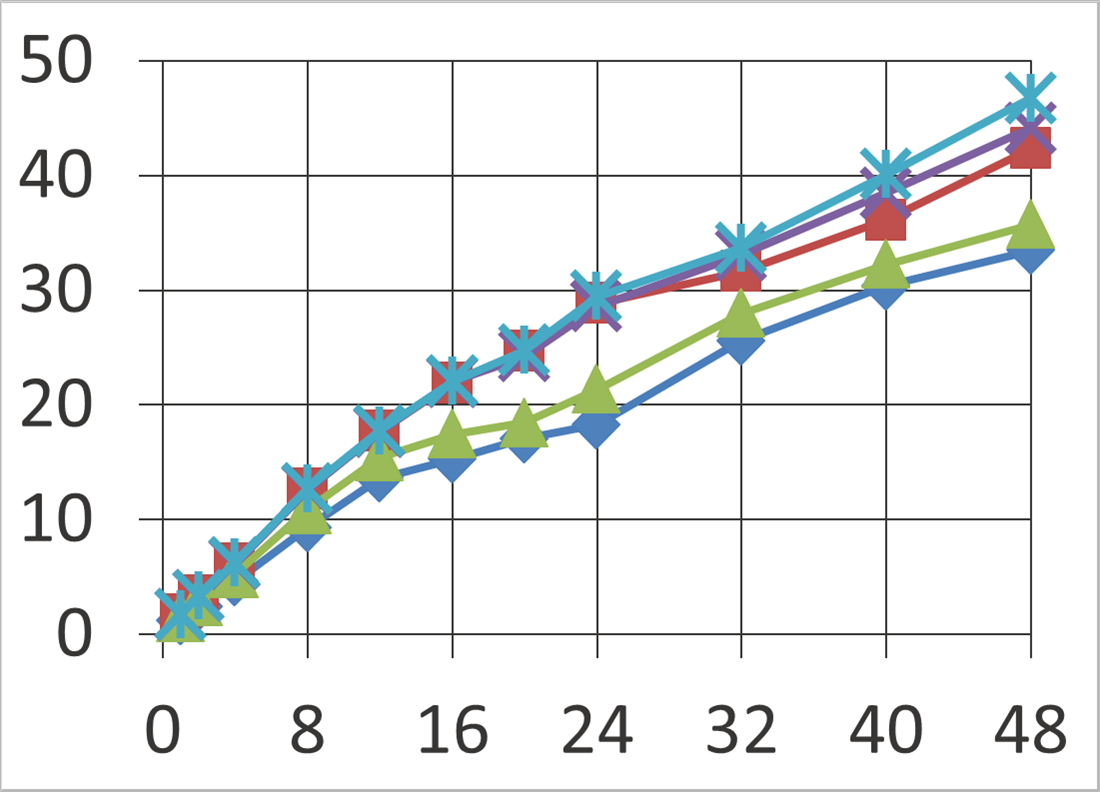
\includegraphics[width=\linewidth]{figures/graphs/0i0d100000k-nrq0.png} &
        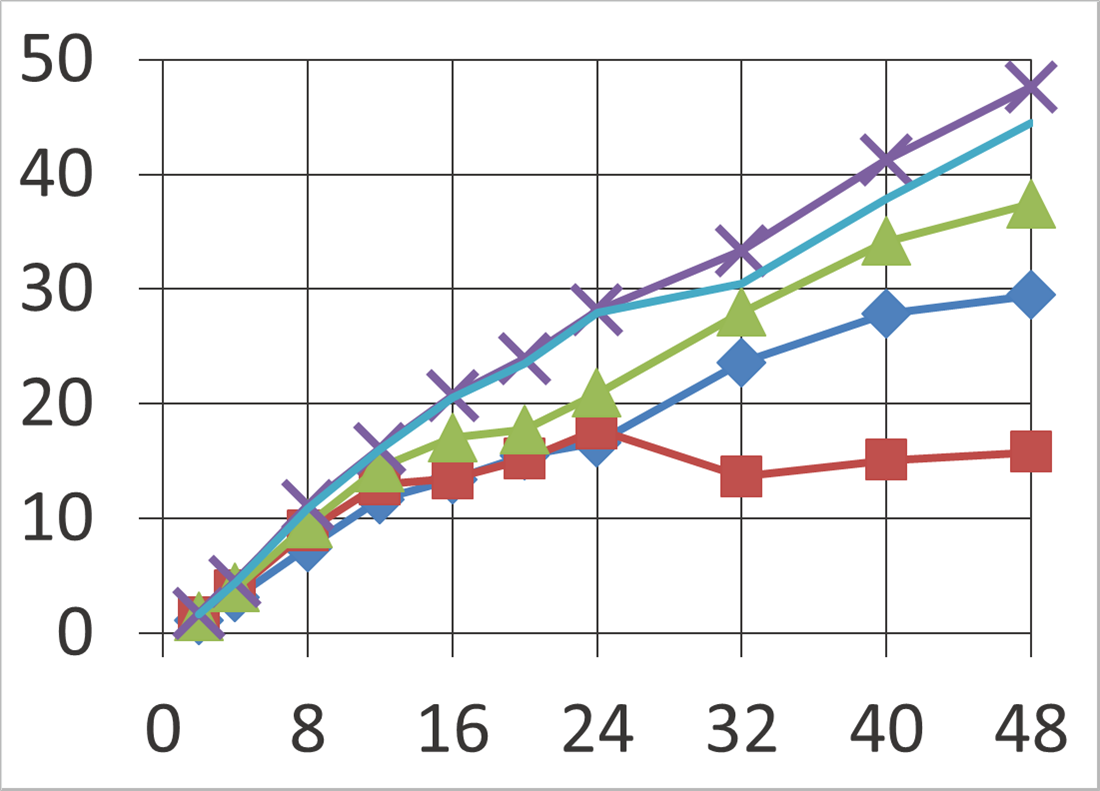
\includegraphics[width=\linewidth]{figures/graphs/0i0d100000k-nrq1.png}
        \\
        \vspace{-5mm}\rotatebox{90}{\small 10\% updates} &
        \vspace{-5mm}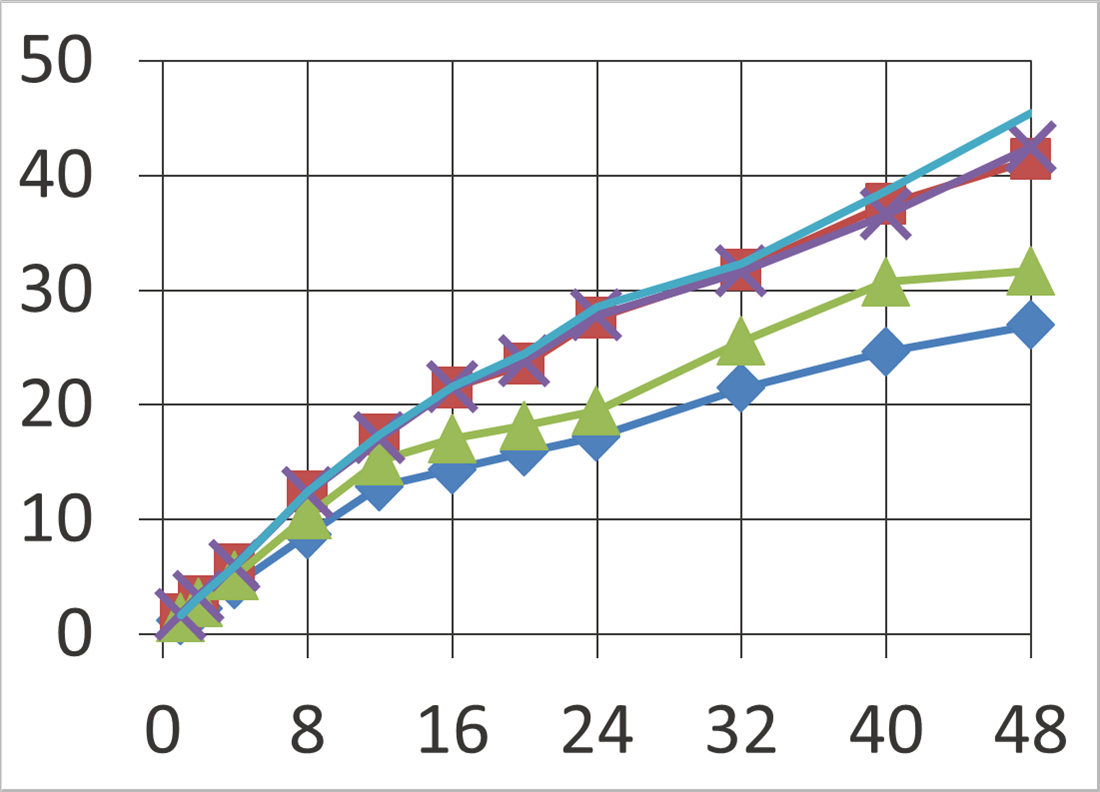
\includegraphics[width=\linewidth]{figures/graphs/5i5d100000k-nrq0.png} &
        \vspace{-5mm}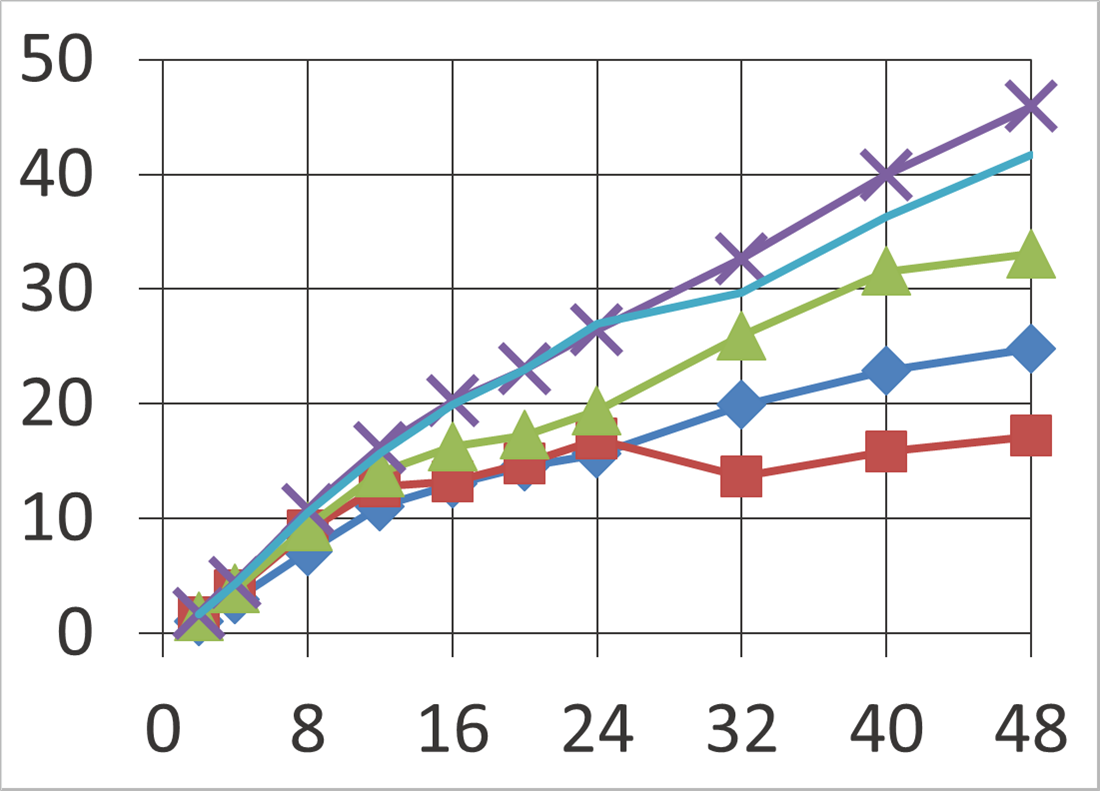
\includegraphics[width=\linewidth]{figures/graphs/5i5d100000k-nrq1.png}
        \\
        \vspace{-5mm}\rotatebox{90}{\small 40\% updates} &
        \vspace{-5mm}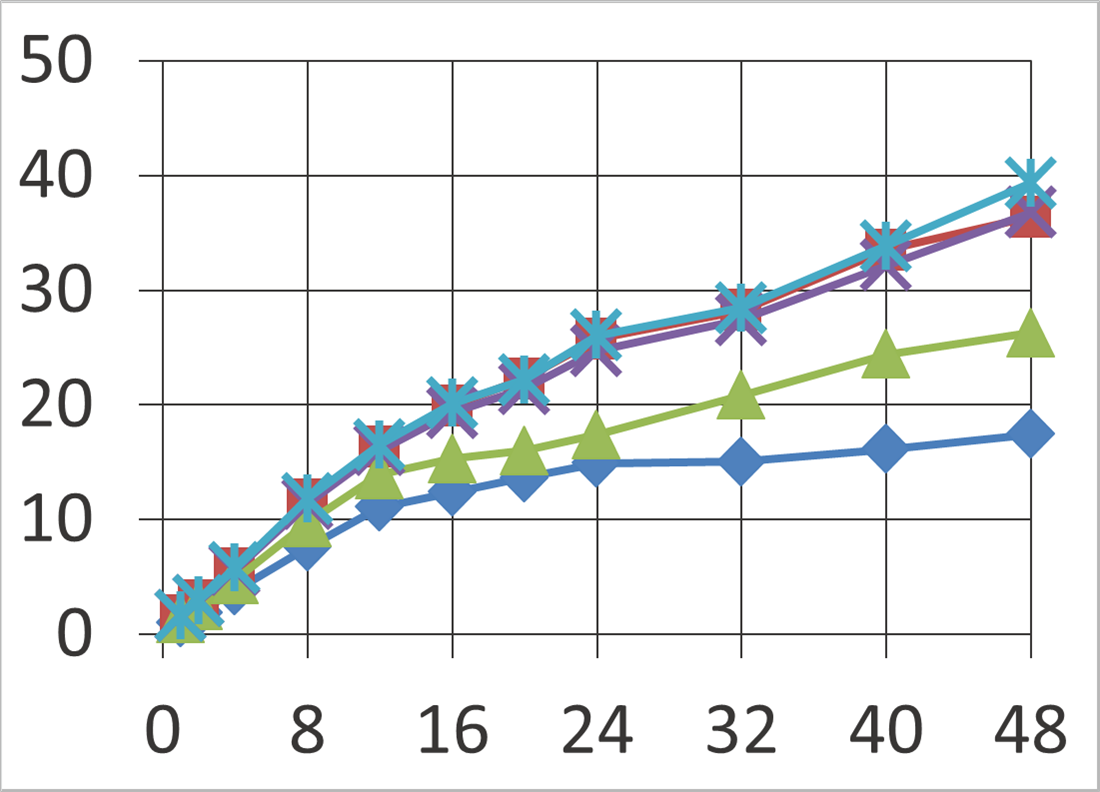
\includegraphics[width=\linewidth]{figures/graphs/20i20d100000k-nrq0.png} &
        \vspace{-5mm}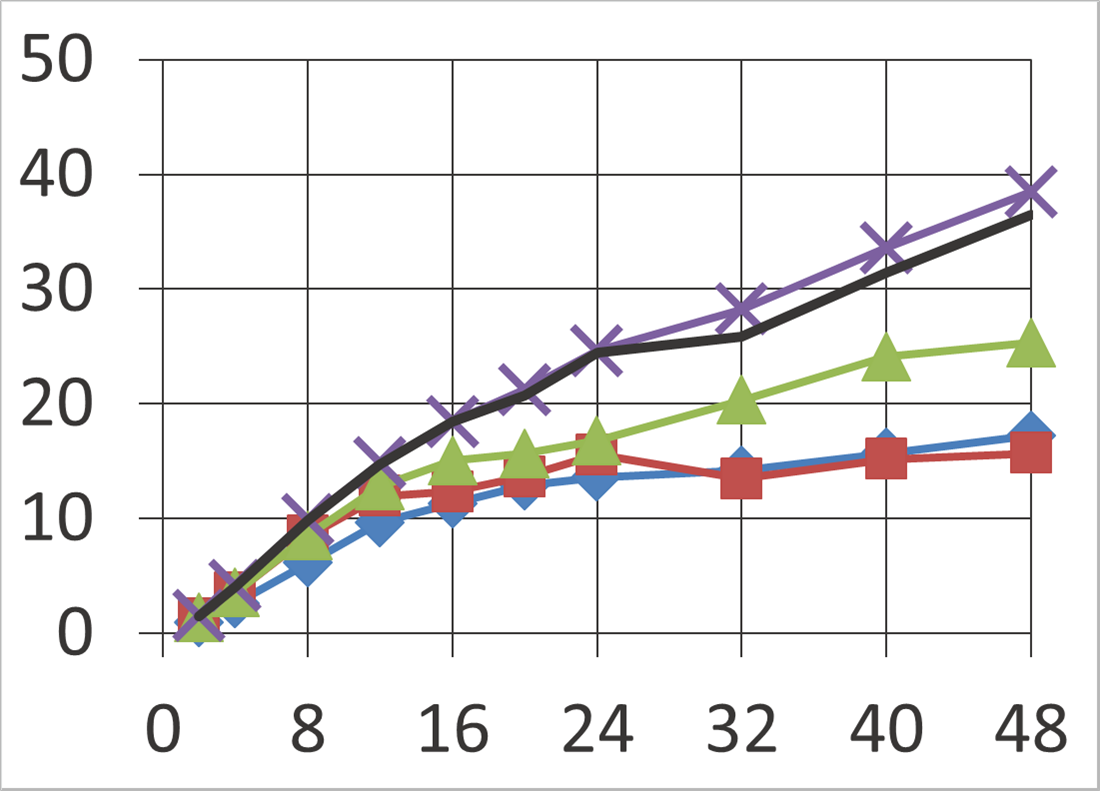
\includegraphics[width=\linewidth]{figures/graphs/20i20d100000k-nrq1.png}
        \\
    \end{tabular}
\end{minipage}
\begin{minipage}{0.495\linewidth}
    \centering
    \textbf{2x12-core IBM POWER8}
    \begin{tabular}{m{0.04\linewidth}m{0.48\linewidth}m{0.48\linewidth}}
        &
        \fcolorbox{black!50}{black!20}{\parbox{\dimexpr \linewidth-2\fboxsep-2\fboxrule}{\centering {\footnotesize No threads perform \textit{RangeIncrement} (W1)}}} &
        \fcolorbox{black!50}{black!20}{\parbox{\dimexpr \linewidth-2\fboxsep-2\fboxrule}{\centering {\footnotesize One thread performs \textit{RangeIncrement} (W2)}}}
        \\
        \rotatebox{90}{\small 0\% updates} &
        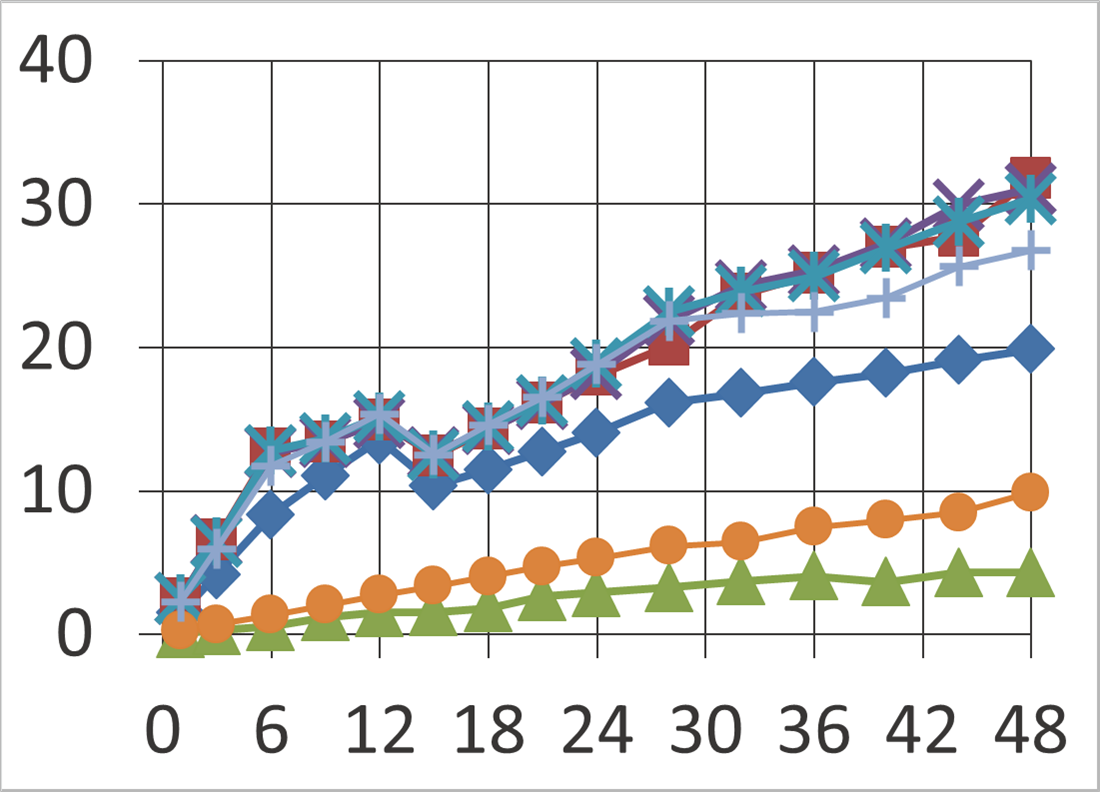
\includegraphics[width=\linewidth]{figures/graphs/power8/0i0d10000k-nrq0.png} &
        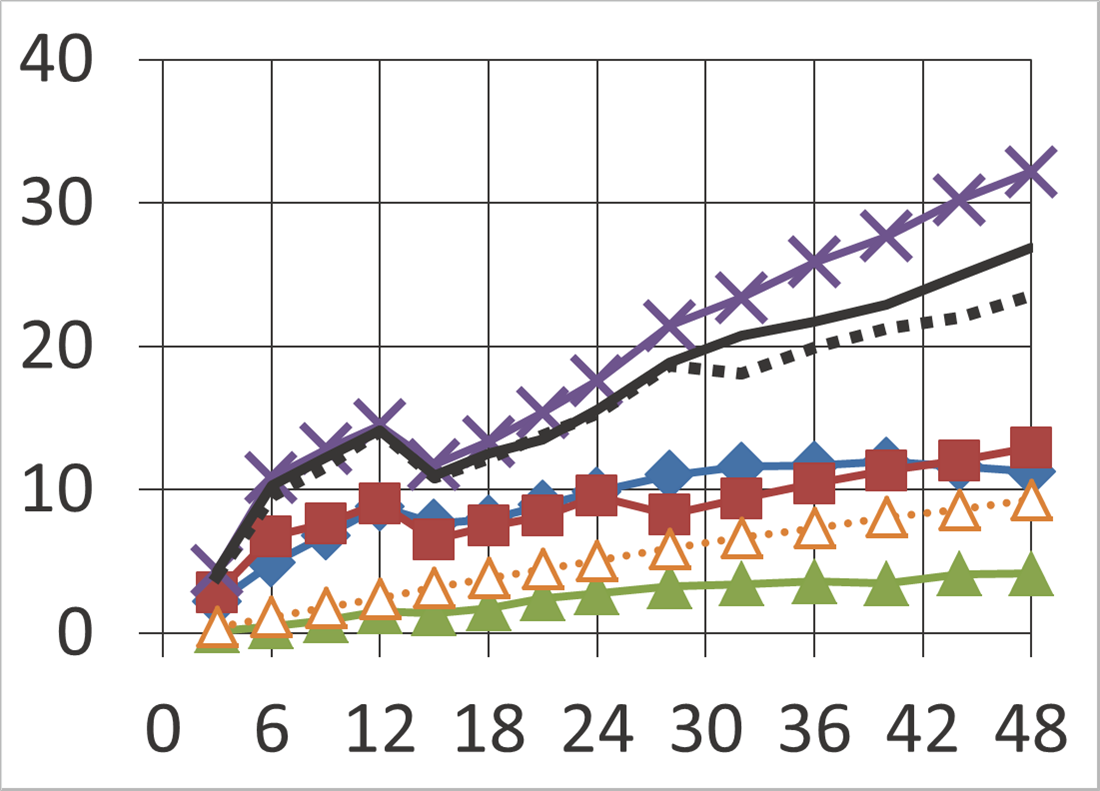
\includegraphics[width=\linewidth]{figures/graphs/power8/0i0d10000k-nrq1.png}
        \\
        \vspace{-5mm}\rotatebox{90}{\small 10\% updates} &
        \vspace{-5mm}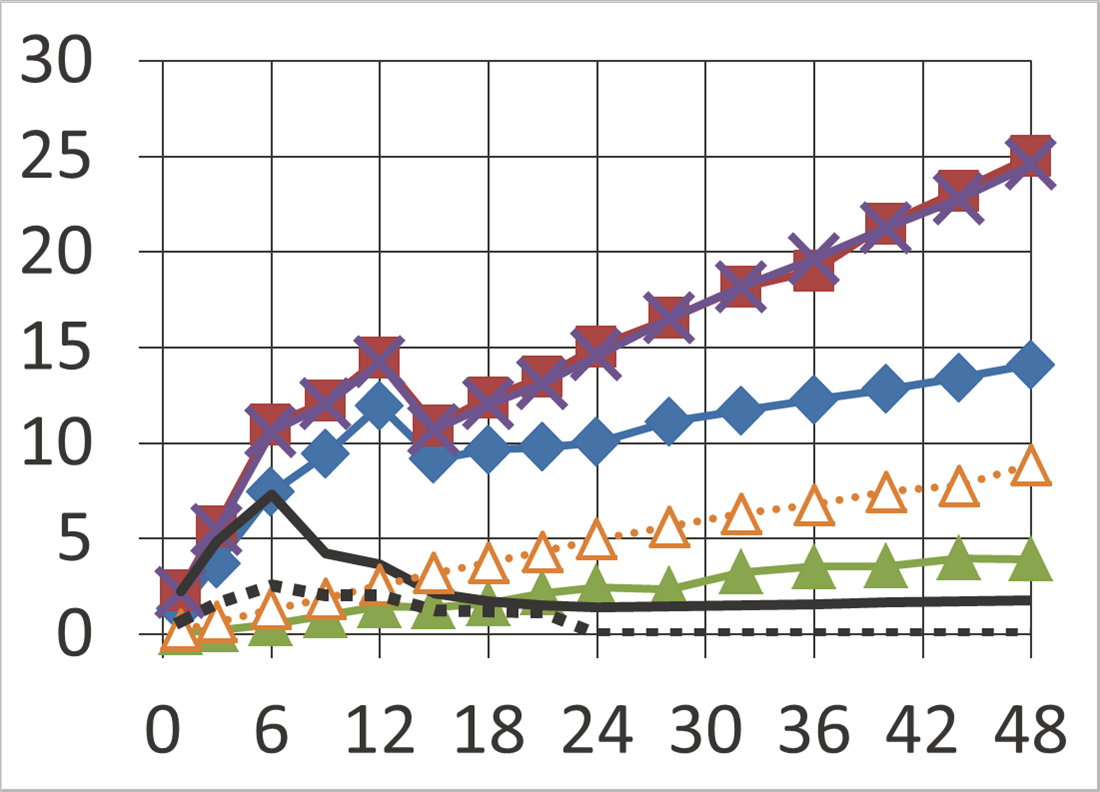
\includegraphics[width=\linewidth]{figures/graphs/power8/5i5d10000k-nrq0.png} &
        \vspace{-5mm}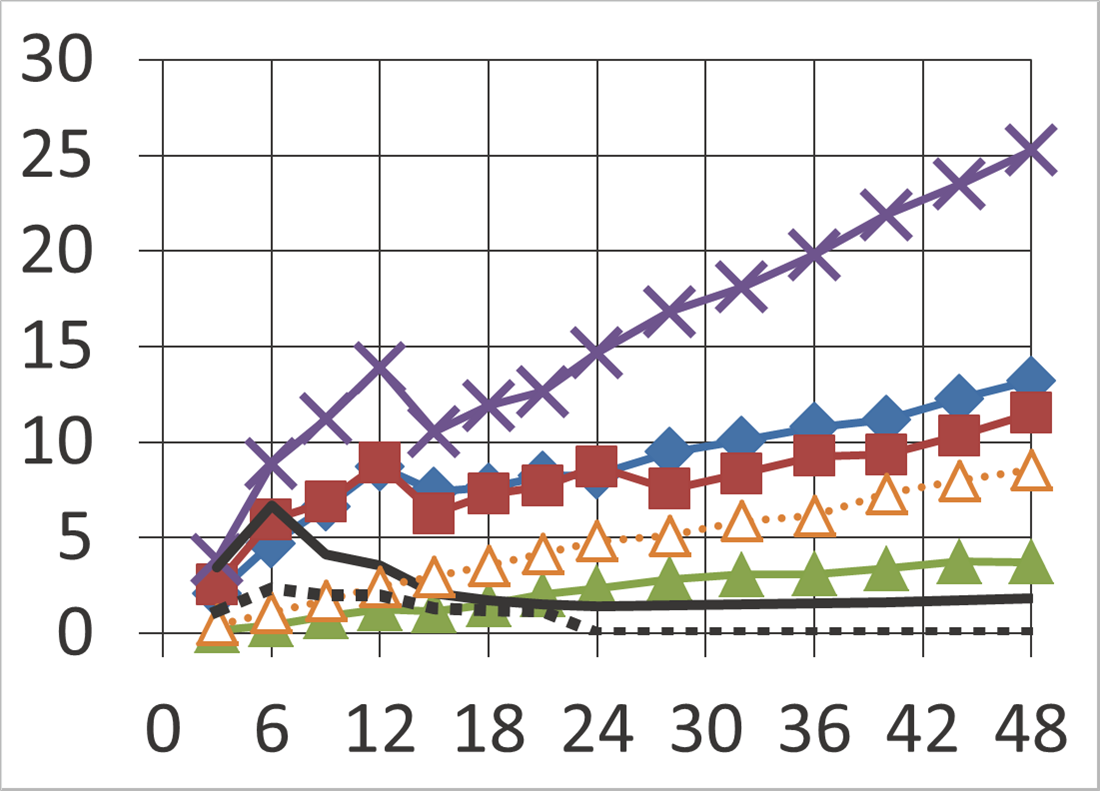
\includegraphics[width=\linewidth]{figures/graphs/power8/5i5d10000k-nrq1.png}
        \\
        \vspace{-5mm}\rotatebox{90}{\small 40\% updates} &
        \vspace{-5mm}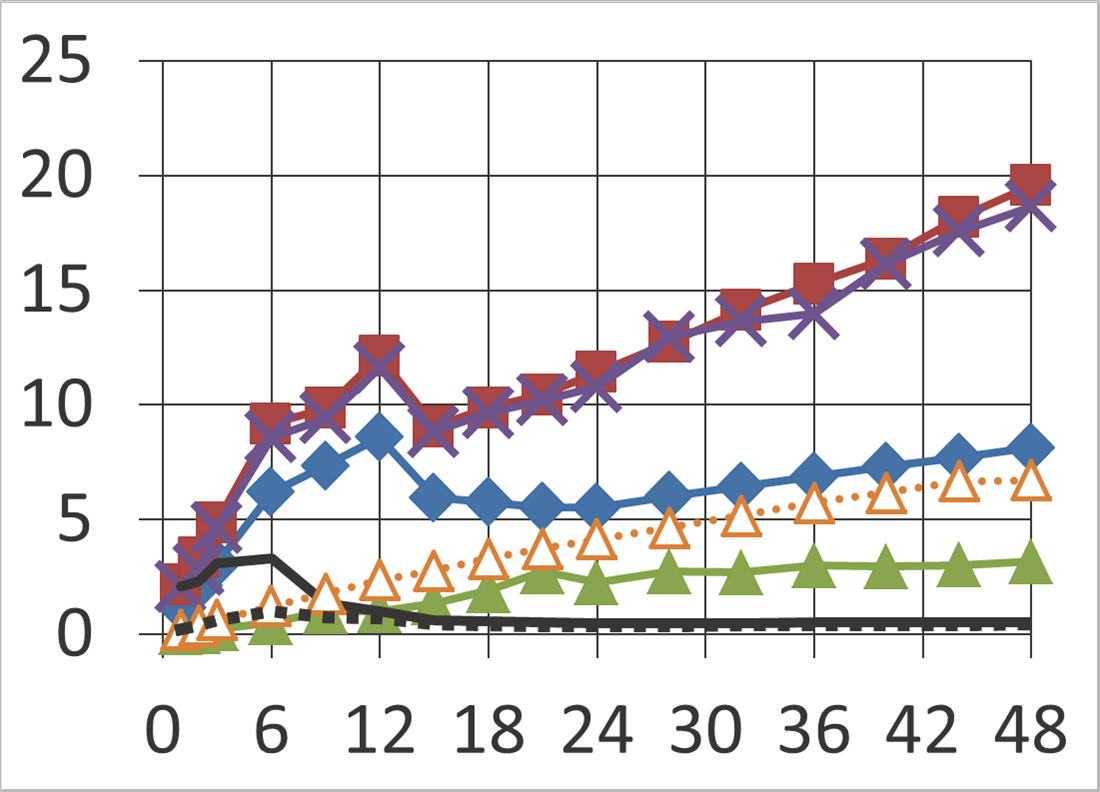
\includegraphics[width=\linewidth]{figures/graphs/power8/20i20d10000k-nrq0.png} &
        \vspace{-5mm}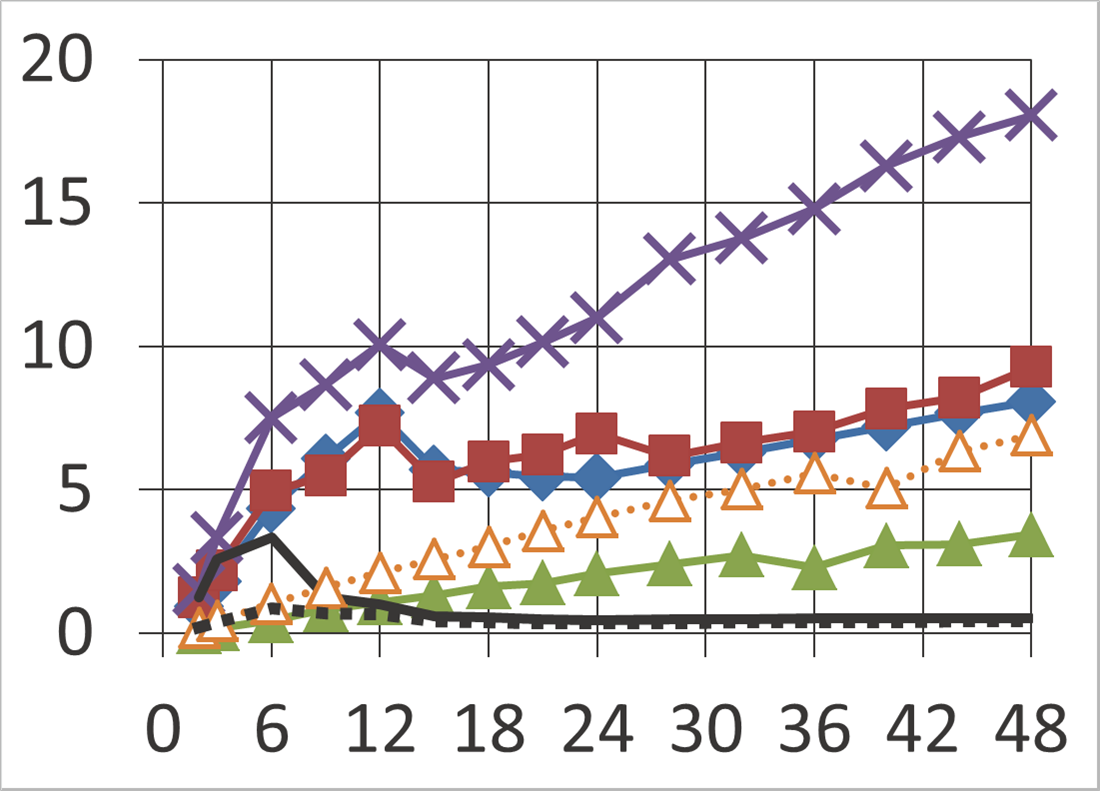
\includegraphics[width=\linewidth]{figures/graphs/power8/20i20d10000k-nrq1.png}
        \\
    \end{tabular}
\end{minipage}
    \vspace{-2mm}
	
\includegraphics[width=\linewidth]{figures/graphs/power8/dsbench3_legend_power.png}
    \vspace{-4mm}
\caption{Results for a \textbf{BST microbenchmark}.
The x-axis represents the number of concurrent threads.
The y-axis represents operations per microsecond.}
\label{fig-exp-bst}
\end{figure}

\vspace{1mm}\noindent\textbf{Results (Intel).}
We first discuss the 0\% updates graph for workload type W1.
In this graph, essentially all operations committed in hardware.
In fact, in each trial, a small fraction of 1\% of operations ran on the slow-path.
Thus, any performance differences shown in the graph are essentially differences in the performance of the algorithms' respective fast-paths (with the exception of TL2).
Algorithm~\ref{alg:inswrite}, which has instrumentation in its fast-path read operations, has significantly lower performance than Algorithm~\ref{alg:inswrite2}, which does not.
Since this is a read-only workload, this instrumentation is responsible for the performance difference.

In the W1 workloads, TLE, Algorithm~\ref{alg:inswrite2} and Hybrid NOrec perform similarly (with a small performance advantage for Hybrid NOrec at high thread counts).
This is because the fast paths for these three algorithms have similar amounts of instrumentation.
In each algorithm, there is no instrumentation for reads or writes, 
and the transaction itself incurs one or two metadata accesses.

In contrast, in the W2 workloads, TLE performs quite poorly, compared to the HyTM algorithms.
In these workloads, transactions must periodically run on the slow-path, and in TLE, 
this entails acquiring a global lock that restricts progress for all other threads.
At high thread counts this significantly impacts performance.
Its performance decreases as the sizes of the ranges passed to \textit{RangeIncrement} increase.
Its performance is also negatively impacted by NUMA effects at thread counts higher than 24.
(This is because, when a thread $p$ reads the lock and incurs a cache miss, 
if the lock was last held by another thread on the same socket, 
then $p$ can fill the cache miss by loading it from the shared L3 cache.
However, if the lock was last held by a thread on a different socket, 
then $p$ must read the lock state from main memory, which is significantly more expensive.)

On the other hand, in each graph in the W2 workloads, the performance of each HyTM (and TL2) is similar to its performance in the corresponding graph in the W1 workloads.
For Algorithm~\ref{alg:inswrite} (and TL2), this is because it is progressive.
Although Algorithm~\ref{alg:inswrite2} is not truly progressive, fast-path transactions will abort only if they are concurrent with the commit procedure of a slow-path transaction.
In \textit{RangeIncrement} operations, there is a long read-only prefix (which is exceptionally long because of Algorithm~\ref{alg:inswrite2}'s quadratic validation) followed by a relatively small set of writes.
Thus, \textit{RangeIncrement} operations have relatively little impact on the fast-path.
The explanation is similar for Hybrid NOrec (except that it performs less validation than Algorithm~\ref{alg:inswrite2}).

Observe that the performance of Hybrid NOrec decreases slightly, relative to Algorithm~\ref{alg:inswrite2}, after 24 threads.
Recall that, in Hybrid NOrec, the global sequence number is a single point of contention on the fast-path.
(In Algorithm~\ref{alg:inswrite2}, the global lock is only modified by slow-path transactions, so fast-path transactions do not have a single point of contention.)
We believe this is due to NUMA effects, similar to those described in~\cite{BKLL16}.
Specifically, whenever a threads on the first socket performs a fast-path transaction that commits and modifies the global lock, it causes cache invalidations for all other threads.
Threads on socket two must then load the lock state from main memory, which takes much longer than loading it from the shared L3 cache.
This causes the transaction to run for a longer time, which lengthens its window of contention, making it more likely to abort.
(Note that, in the 0\% updates graph in the W2 workload, we still see this effect, because there is a thread performing \textit{RangeIncrement} operations.)
%% IF THIS DISCREPANCY IS DUE TO NUMA EFFECTS HURTING UPDATES, WHY DOES THE GAP BETWEEN ALGORITHMS DECREASE AS THE NUMBER OF UPDATES INCREASES?
% here's a subtle hypothesis. there are two different numa effects competing to be the dominating performance factor. one is the effect i just described above. the other is the negative performance impact of tree updates on traversals. this is something we saw in the oracle spaa paper when looking at tree updates in htm. i expect that the strength of the negative numa effects on tree traversals with increased updates is greater than the strength of the negative numa effects of esl and gsl updates. since the negative effects on tree traversals impact both algorithms, it makes the difference in performance less significant, masking the other numa effect.

\vspace{1mm}\noindent\textbf{Results (IBM Power8).}
%
Algorithm~\ref{alg:inswrite} performs poorly on Power8: Power8 transactions can only load 64 cache lines before they will abort~\cite{nguyen-thesis}. 
Transactions read locks and tree nodes, which are in different cache lines: together, they often exceed 64 cache lines loaded in a tree operation, 
so most transactions cannot succeed in hardware. Consequently, on Power8, 
it is incredibly important either to have minimal instrumentation in transactions, or for metadata to be located in the 
same cache lines as program data. Of course, the latter is not possible for HyTMs, which do not have control over the layout of program data.
Consequently, Algorithm~\ref{alg:inswrite2} outperforms Algorithm~\ref{alg:inswrite} in Power8 quite easily by avoiding the per-read instrumentation. 

Algorithm~\ref{alg:inswrite} is improved by suspend/resume on sequence locks, but suspend/resume instructions are expensive on Power8, 
so it still performs relatively poorly. 
To make suspend/resume a practical tool, one could imagine attempting to 
collect several metadata accesses and perform them together to amortize the cost of a suspend/resume pair. For instance, 
in Algorithm~\ref{alg:inswrite}, one might try to update the locks for all of a transactions writes at once, when the transaction commits. 
Typically one would accomplish this by logging all writes so that a process can remember which addresses it must lock at commit time. 
however, logging the writes inside the transaction would be at least as costly as just performing them.

Observe that Hybrid NOrec does far worse with updates in Power8 than on the Intel machine.
This is due to the fact that fetch-increment on a single location experiences severe negative scaling on the Power8 processes: e.g., in one second, a single
thread can perform 37 fetch-add operations while 6 threads perform a total of 9 million and 24 threads perform only 4 million fetch-add operations.
In contrast, the Intel machine performs 32 million operations with 6 threads and 45 million with 24 threads. This is likely because this Intel processor provides 
fetch-add instructions while it must be emulated on the Power8 processor (using load-linked/store-conditional).

In Hybrid NOrec\textsuperscript{$\ast$}, the non-speculative increment of gsl actually makes performance worse. Recall that in Hybrid NOrec, 
if a fast path transaction $T_1$ increments gsl, and then a software transaction $T_2$ reads gsl (as part of validation) before $T_1$ commits, then $T_1$ will abort, 
and $T_2$ will not see $T_1$'s change to gsl. 
So, $T_2$ will have a higher chance of avoiding incremental validation (and, hence, will likely take less time to run, and have a smaller contention window). 
However, in Hybrid NOrec\textsuperscript{$\ast$}, once $T_1$ increments gsl, $T_2$ will see the change to gsl, regardless of whether $T_1$ commits or aborts. Thus, 
$T_2$ will be forced to perform incremental validation. In our experiments, we observed that a much larger number of transactions ran on 
the fallback path in Hybrid NOrec\textsuperscript{$\ast$} than in Hybrid NOrec (often several orders of magnitude more).
